\chapter{अभिक्रिया दरें}\label{ch:g12:reaction-rates}

रसोई के काउंटर पर छोड़ी गई दूध की बोतल दो-एक दिन में खट्टी हो जाती है;
फ्रिज में वह एक हफ़्ते से ज़्यादा टिकी रहती है। आतिशबाज़ी पल भर के एक अंश में
जल जाती है, जबकि शहर के किसी पार्क में चूना-पत्थर की मूर्ति सदियों में
घिसती है। \omterm{def:g8:balanced-equations:equation}{संतुलित समीकरण} और \omterm{def:g10:reaction-progress-table:extent}{प्रगति सारणियाँ} बताती हैं कि कोई
अभिक्रिया क्या और कितना देती है; वे यह कुछ नहीं बतातीं कि कितनी तेज़ी से। यह
अध्याय अभिक्रियाओं की चाल मापता है, खोजता है कि उसे क्या नियंत्रित करता है, और
उस सबसे सरल ढंग का वर्णन करता है जिससे कोई अभिक्रिया चलते-चलते धीमी पड़ सकती है।

\begin{recall}
किसी विलयन की सांद्रता (\cref{ch:g10:concentration-and-dilution})
और किसी \omterm{def:g10:reaction-progress-table:extent}{अभिक्रिया की प्रगति} (\cref{ch:g10:reaction-progress-table})। किसी तनु
विलयन की \omterm{def:g11:absorbance:absorbance}{अवशोषकता} रंगीन स्पीशीज़ की सांद्रता के
समानुपाती होती है (\cref{ch:g11:absorbance})। \omterm{def:g11:titration:titration}{अनुमापन} किसी
स्पीशीज़ की मात्रा मापता है (\cref{ch:g11:titration})।
\end{recall}

\begin{omfigure}
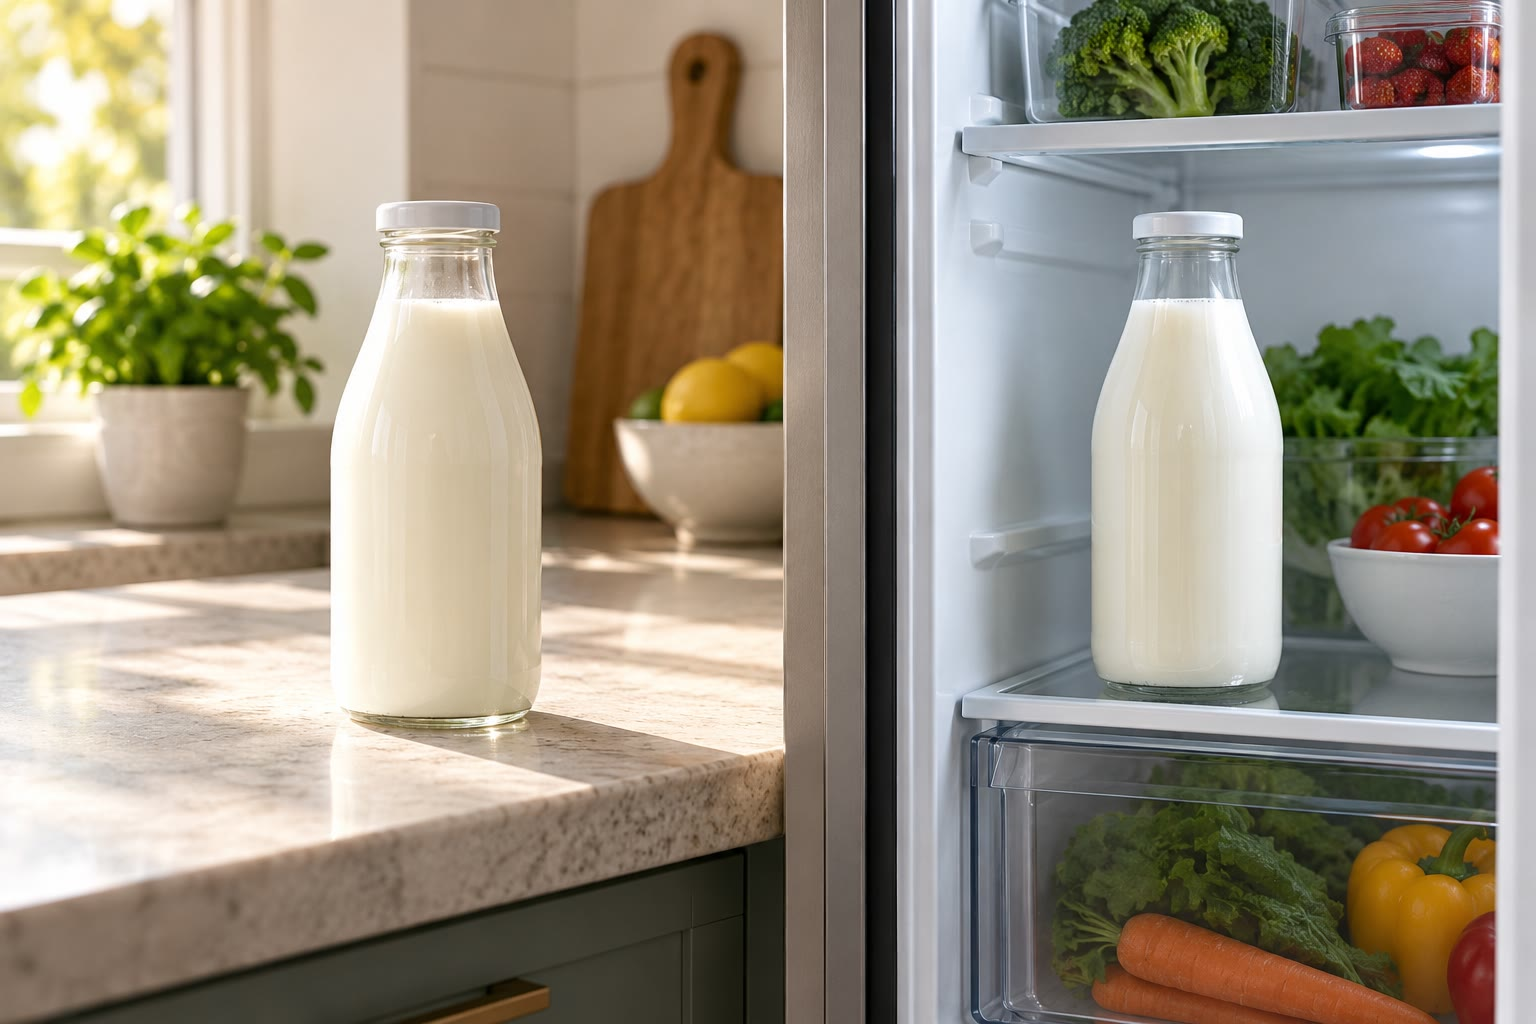
\includegraphics[width=0.48\linewidth]{images/book1/ai/g12-milk-counter-fridge.jpg}

{\small वही दूध, काउंटर पर और फ्रिज में: उसे खट्टा करने वाली अभिक्रियाएँ
ठंड में धीमी होती हैं।}
\end{omfigure}

\section{समय के साथ किसी अभिक्रिया पर नज़र रखना}

कुछ अभिक्रियाएँ \omterm{def:g7:chemical-reactions:reactant}{अभिकारकों} के मिलते ही पूरी हो जाती हैं: सिल्वर क्लोराइड का
\omterm{def:g9:ions:precipitate}{अवक्षेपण}, किसी अम्ल की किसी क्षारक से अभिक्रिया। दूसरी अभिक्रियाओं में
मिनट, घंटे या वर्ष लगते हैं। किसी धीमी अभिक्रिया का अध्ययन करने के लिए रसायनज्ञ
नियमित समयों पर किसी \omterm{def:g7:chemical-reactions:reactant}{अभिकारक} या उत्पाद की सांद्रता मापते हैं। वे
\begin{itemize}
  \item छोटे नमूने ले सकते हैं, हर एक में अभिक्रिया रोक सकते हैं, और उनका \omterm{def:g11:titration:titration}{अनुमापन} कर सकते हैं;
  \item विलयन की \omterm{def:g11:absorbance:absorbance}{अवशोषकता} माप सकते हैं, जब कोई \omterm{def:g7:chemical-reactions:reactant}{अभिकारक} या
        उत्पाद रंगीन हो;
  \item निकलने वाली गैस का दाब या आयतन माप सकते हैं, या ऐसे विलयन की
        चालकता जिसके \omterm{def:g9:ions:ion}{आयन} बदलते हैं।
\end{itemize}

\begin{definition}[शमन]\label{def:g12:reaction-rates:quenching}
किसी नमूने का \emph{शमन}\index{शमन} लेने के क्षण ही उसमें अभिक्रिया को रोकना,
या बहुत अधिक धीमा करना है, आम तौर पर उसे अचानक ठंडा करके और
तनु करके, ताकि उसकी संरचना आराम से
मापी जा सके।
\end{definition}

\begin{inthelab}[किसी नमूने का शमन]
हर पाँच मिनट पर अभिक्रिया \omterm{def:g6:pure-substances-and-mixtures:mixture}{मिश्रण} के \qty{10.0}{mL} पिपेट से
लिए जाते हैं और लगभग \qty{40}{mL} बर्फ़-ठंडे पानी वाले बीकर में
डाले जाते हैं। पाँच गुना तनु और लगभग
\qty{0}{\celsius} तक ठंडा होने पर अभिक्रिया इतनी धीमी हो जाती है कि उसे
रुकी हुई माना जा सकता है; फिर नमूने का \omterm{def:g11:titration:titration}{अनुमापन} किया जाता है। नमूने का समय
वह समय है जब उसे बर्फ़ीले पानी में डाला गया, \omterm{def:g11:titration:titration}{अनुमापन} का समय नहीं।
\end{inthelab}

\begin{omfigure}
\begin{tikzpicture}[font=\small, scale=0.8]
  \pic[transform shape] at (0,0) {erlenmeyer={0.4}{orange!25}};
  \node[anchor=north, align=center] at (0,-0.15) {अभिक्रिया\\ मिश्रण};
  \pic[transform shape, rotate=-35] at (1.4,1.2) {pipette={0.6}{orange!25}};
  \draw[omProp, very thick, -{Stealth}] (1.6,0.8) -- (2.9,0.8);
  \node[anchor=south] at (2.25,0.85) {\qty{10.0}{mL}};
  \pic[transform shape] at (4,0) {beaker={0.55}{cyan!12}};
  \foreach \p in {(3.6,0.4),(4.2,0.6),(3.9,0.85),(4.4,0.3)}
    \draw[black!30, fill=white] \p ++(-0.1,-0.08) rectangle ++(0.2,0.16);
  \node[anchor=north, align=center] at (4,-0.15) {बर्फ़-ठंडा पानी:\\ अभिक्रिया रुकी};
  \draw[omProp, very thick, -{Stealth}] (5.1,0.8) -- (6.4,0.8);
  \pic[transform shape] at (7.5,0) {erlenmeyer={0.35}{orange!12}};
  \pic[transform shape] at (7.5,2.75) {burette={0.7}{violet!45}};
  \node[anchor=north, align=center] at (7.5,-0.15) {नमूने का\\ अनुमापन};
\end{tikzpicture}

{\small नमूने लेकर किसी अभिक्रिया पर नज़र रखना: नमूना लीजिए, उसका \omterm{def:g12:reaction-rates:quenching}{शमन} कीजिए, फिर
उसे आराम से मापिए।}
\end{omfigure}

\section{गतिक कारक}

\begin{definition}[गतिक कारक]\label{def:g12:reaction-rates:kinetic-factor}
\emph{गतिक कारक}\index{गतिक कारक} वह राशि है जो किसी अभिक्रिया की
चाल बदलती है, बिना यह बदले कि अभिक्रिया क्या देती है: ताप,
\omterm{def:g7:chemical-reactions:reactant}{अभिकारकों} की सांद्रताएँ, भिन्न प्रावस्थाओं वाले \omterm{def:g7:chemical-reactions:reactant}{अभिकारकों} के बीच संपर्क का
क्षेत्रफल, और उत्प्रेरक की उपस्थिति
(अगला अध्याय)।
\end{definition}

\begin{proposition}[अधिक गरम, अधिक सांद्र, अधिक बारीक: अधिक तेज़]\label{prop:g12:reaction-rates:factors}
सामान्यतः कोई अभिक्रिया तब तेज़ होती है जब ताप अधिक हो, जब
\omterm{def:g7:chemical-reactions:reactant}{अभिकारक} अधिक सांद्र हों, और, ठोस \omterm{def:g7:chemical-reactions:reactant}{अभिकारक} के लिए, जब वह
अधिक बारीक पिसा हो।
\end{proposition}

\begin{proof}
एक चित्र के साथ स्वीकृत: अभिक्रिया करने वाले कणों को मिलना चाहिए, और पर्याप्त
ज़ोर से मिलना चाहिए। उन्हें सांद्र करने से मिलन अधिक बार होते हैं; ठोस को बारीक करने
से मिलने के लिए अधिक सतह मिलती है; गरम करने से वे तेज़ चलते हैं, जिससे वे
अधिक बार मिलते हैं और, सबसे बढ़कर, अधिक मिलन आबंध तोड़ने लायक
ऊर्जावान होते हैं।
\end{proof}

\begin{example}[रोज़मर्रा के तीन उदाहरण]\label{ex:g12:reaction-rates:everyday}
भोजन फ्रिज में अधिक समय तक और फ्रीज़र में कहीं अधिक समय तक टिकता है:
उसे ख़राब करने वाली अभिक्रियाएँ ठंड में धीमी पड़ जाती हैं। चक्की की \omterm{def:g4:air-a-mixture-of-gases:air}{हवा} में
आटे की बारीक धूल फट सकती है, जबकि आटे की बोरी केवल सुलगती है: वही
अभिक्रिया, संपर्क का विशाल क्षेत्रफल। पानी में बुदबुदाने वाली गोली
पहले पीस ली जाए तो अधिक तेज़ी से \omterm{def:g2:mixing-and-dissolving:dissolve}{घुलती} है।
\end{example}

\begin{omfigure}
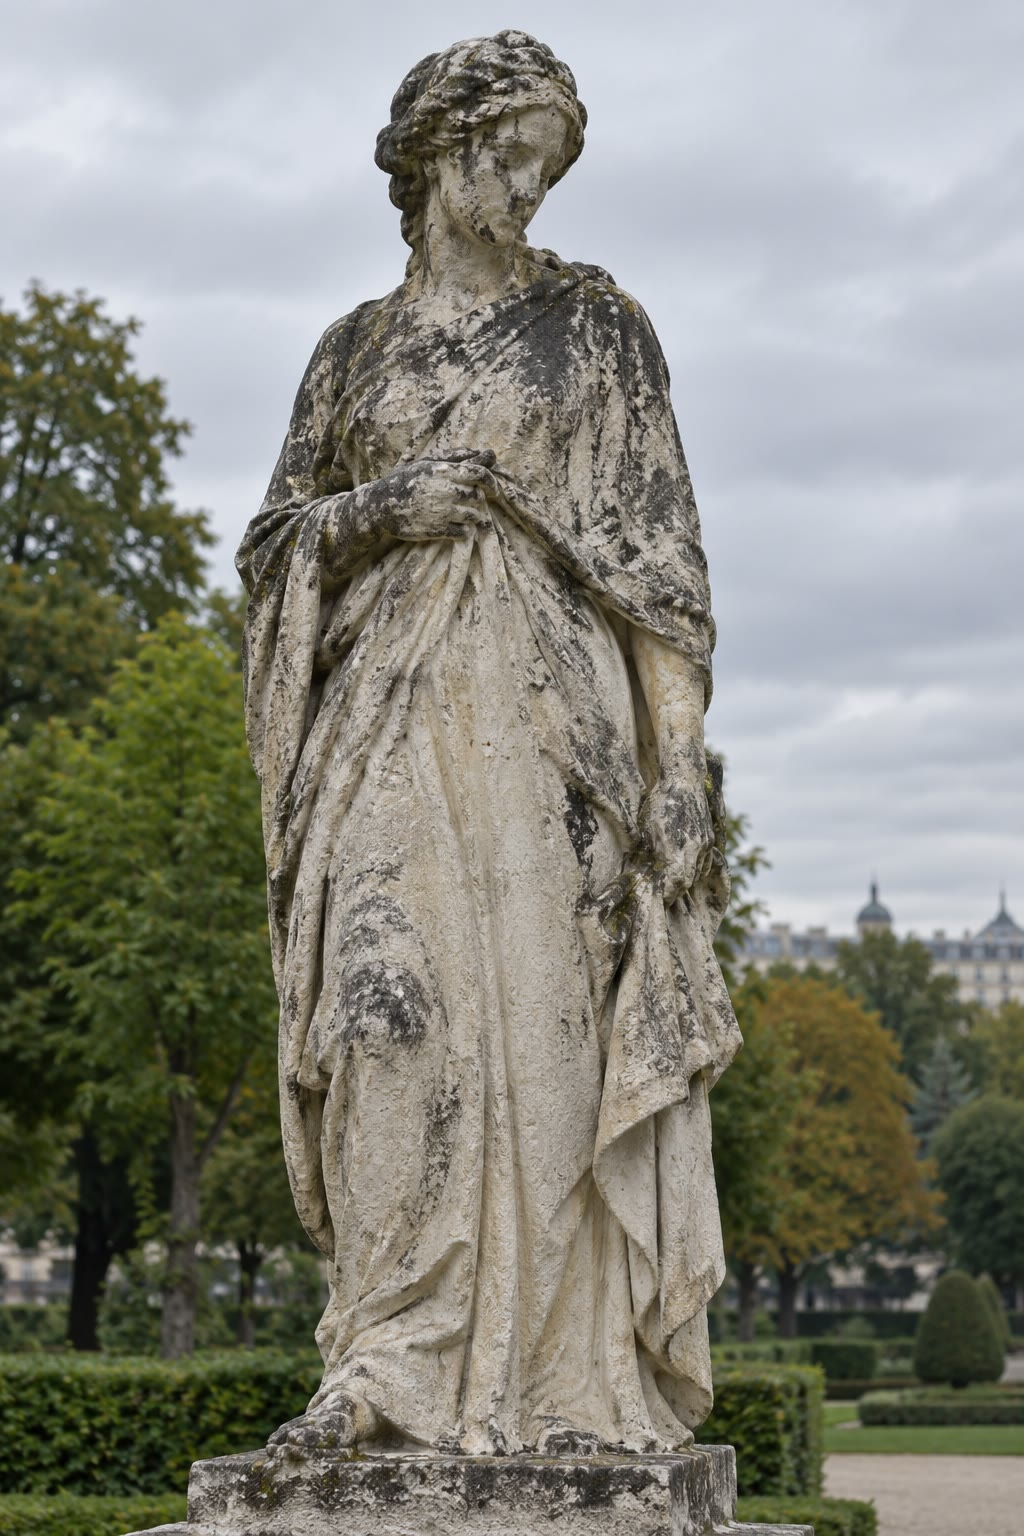
\includegraphics[width=0.42\linewidth,height=6cm,keepaspectratio]{images/book1/ai/g12-weathered-statue.jpg}

{\small वर्षा से घिसी चूना-पत्थर की एक मूर्ति: एक अभिक्रिया जिसमें
सदियाँ लगती हैं।}
\end{omfigure}

\section{लोप दर और प्रकटन दर}

\begin{definition}[लोप दर, प्रकटन दर]\label{def:g12:reaction-rates:rate}
स्थिर आयतन वाले विलयन में समय $t$ पर किसी \omterm{def:g7:chemical-reactions:reactant}{अभिकारक} A की \emph{लोप दर}\index{लोप दर}
है
\[
  v_A(t) = -\frac{d[\ce{A}]}{dt},
\]
और किसी उत्पाद P की \emph{प्रकटन दर}\index{प्रकटन दर}
$v_P(t) = \dfrac{d[\ce{P}]}{dt}$ है। दोनों धनात्मक हैं,
\si{mol.L^{-1}.min^{-1}} (या प्रति सेकंड) में।
\end{definition}


\begin{method}[स्पर्शरेखा से दर पढ़ना]\label{met:g12:reaction-rates:tangent}
\begin{enumerate}
  \item $[\ce{A}]$ बनाम $t$ के वक्र पर चुने गए समय पर
        स्पर्शरेखा खींचिए।
  \item स्पर्शरेखा पर दूर-दूर के दो बिंदु पढ़िए और उसकी प्रवणता
        $\Delta[\ce{A}] / \Delta t$ निकालिए।
  \item \omterm{def:g12:reaction-rates:rate}{लोप दर} इस प्रवणता का ऋणात्मक है (किसी
        उत्पाद के लिए, स्वयं प्रवणता)।
\end{enumerate}
\end{method}

\begin{omfigure}
\begin{tikzpicture}
\begin{axis}[width=0.8\linewidth, height=6.4cm, xmin=0, xmax=60, ymin=0,
    ymax=11, xlabel={$t$ (\si{min})}, ylabel={$[\ce{A}]$ (\si{mmol/L})},
    axis lines*=left, ymajorgrids, xmajorgrids, grid style={gray!20},
    tick label style={font=\small}, label style={font=\small},
    legend style={font=\small, at={(0.98,0.97)}, anchor=north east,
    draw=none, fill=white}, legend cell align=left]
  \addplot[very thick, omDef] table[x=t, y=A1] {figdata/out/grade-12-reaction-rates-a.dat};
  \addplot[very thick, omThm] table[x=t, y=A2] {figdata/out/grade-12-reaction-rates-a.dat};
  \addplot[thick, dashed, omProp, restrict y to domain=0:11] table[x=t, y=tangent]
    {figdata/out/grade-12-reaction-rates-a.dat};
  \legend{$k = \qty{0.050}{min^{-1}}$, $k = \qty{0.100}{min^{-1}}$ (अधिक गरम),
    $t = 0$ पर स्पर्शरेखा}
  \addplot[densely dotted, black!60] coordinates {(0,5) (13.86,5) (13.86,0)};
  \addplot[densely dotted, black!60] coordinates {(6.93,5) (6.93,0)};
  \node[font=\small, anchor=south west] at (axis cs:14.6,5.4) {$t_{1/2} = \qty{13.9}{min}$};
  \node[font=\small, anchor=south east] at (axis cs:6.7,0.2) {\qty{6.9}{min}};
\end{axis}
\end{tikzpicture}

{\small एक ही \omterm{def:g12:reaction-rates:first-order}{प्रथम कोटि की अभिक्रिया} के लिए, दो तापों पर, समय के विरुद्ध किसी \omterm{def:g7:chemical-reactions:reactant}{अभिकारक} A
की सांद्रता। $t = 0$ पर स्पर्शरेखा (डैश वाली)
प्रारंभिक दर देती है; बिंदुदार रेखाएँ \omterm{def:g12:reaction-rates:half-life}{अर्ध-आयु} दर्शाती हैं।}
\end{omfigure}

\begin{example}[प्रारंभिक दर]\label{ex:g12:reaction-rates:initial}
नीले वक्र पर $t = 0$ पर स्पर्शरेखा
$t = 0$ पर \qty{10.0}{mmol/L} से चलकर $0$ तक पहुँचती है, $t = \qty{20}{min}$ के क्षण पर। इसलिए उसकी प्रवणता
$-10.0/20 = \qty{-0.50}{mmol.L^{-1}.min^{-1}}$ है, और प्रारंभिक
\omterm{def:g12:reaction-rates:rate}{लोप दर} \qty{0.50}{mmol.L^{-1}.min^{-1}} है। बाद में वक्र चपटा होता है
और दर घटती है: A के खपने के साथ अभिक्रिया धीमी पड़ती है।
\end{example}

\section{प्रथम कोटि की अभिक्रियाएँ}

\begin{definition}[प्रथम कोटि की अभिक्रिया, दर स्थिरांक]\label{def:g12:reaction-rates:first-order}
कोई अभिक्रिया A के सापेक्ष \emph{प्रथम कोटि की अभिक्रिया}\index{प्रथम कोटि की अभिक्रिया}
है यदि उसकी \omterm{def:g12:reaction-rates:rate}{लोप दर} हर क्षण A की सांद्रता के
समानुपाती हो:
\[
  -\frac{d[\ce{A}]}{dt} = k\,[\ce{A}] .
\]
धनात्मक स्थिरांक $k$, \si{min^{-1}} या \si{s^{-1}} में,
\emph{दर स्थिरांक}\index{दर स्थिरांक} है; वह ताप पर निर्भर करता है।
\end{definition}

\begin{proposition}[चरघातांकी क्षय]\label{prop:g12:reaction-rates:exponential}
प्रारंभिक सांद्रता $[\ce{A}]_0$ वाली \omterm{def:g12:reaction-rates:first-order}{प्रथम कोटि की अभिक्रिया} के लिए,
\[
  [\ce{A}](t) = [\ce{A}]_0\, e^{-kt} .
\]
\end{proposition}

\begin{proof}
फलन $f(t) = [\ce{A}]_0 e^{-kt}$ का अवकलज
$f'(t) = -k [\ce{A}]_0 e^{-kt} = -k f(t)$ है, इसलिए यह दर
समीकरण को संतुष्ट करता है, और $f(0) = [\ce{A}]_0$। यह कि यही एकमात्र ऐसा फलन है,
यहाँ स्वीकार किया गया है (गणित में इसे $y' = ay$ प्रकार के समीकरणों के लिए सिद्ध किया जाता है)।
\end{proof}

\begin{method}[प्रथम कोटि की जाँच]\label{met:g12:reaction-rates:test}
\begin{enumerate}
  \item मापों से हर समय पर $\ln [\ce{A}]$ (या $\ln A$, यदि \omterm{def:g11:absorbance:absorbance}{अवशोषकता}
        $[\ce{A}]$ के समानुपाती हो) निकालिए।
  \item $\ln[\ce{A}]$ बनाम $t$ आलेखित कीजिए: चूँकि
        $\ln[\ce{A}] = \ln[\ce{A}]_0 - kt$, बिंदु एक सीधी
        रेखा पर तभी और केवल तभी होते हैं जब अभिक्रिया प्रथम कोटि की हो।
  \item रेखा की प्रवणता $-k$ है।
\end{enumerate}
\end{method}

\section{अर्ध-आयु}

\begin{definition}[अर्ध-आयु]\label{def:g12:reaction-rates:half-life}
किसी अभिक्रिया की \emph{अर्ध-आयु}\index{अर्ध-आयु} $t_{1/2}$ वह समय है
जिसमें \omterm{def:g10:reaction-progress-table:limiting}{सीमांत अभिकारक} की सांद्रता घटकर अपने प्रारंभिक मान की
आधी रह जाती है।
\end{definition}

\begin{proposition}[प्रथम कोटि की अभिक्रिया की अर्ध-आयु]\label{prop:g12:reaction-rates:half-life}
\omterm{def:g12:reaction-rates:first-order}{प्रथम कोटि की अभिक्रिया} के लिए,
\[
  t_{1/2} = \frac{\ln 2}{k},
\]
प्रारंभिक सांद्रता चाहे जो हो; $n$ \omterm{def:g12:reaction-rates:half-life}{अर्ध-आयुओं} के बाद
सांद्रता $2^n$ से विभाजित हो जाती है।
\end{proposition}

\begin{proof}
$[\ce{A}]_0 e^{-k t_{1/2}} = [\ce{A}]_0 / 2$ से $e^{-k t_{1/2}} = 1/2$ मिलता है,
इसलिए $k t_{1/2} = \ln 2$। हर अगली \omterm{def:g12:reaction-rates:half-life}{अर्ध-आयु}
सांद्रता को फिर से $e^{-k t_{1/2}} = 1/2$ से गुणा करती है।
\end{proof}


\begin{example}[अर्ध-आयु पढ़ना]\label{ex:g12:reaction-rates:half-lives}
$k = \qty{0.050}{min^{-1}}$ के लिए, $t_{1/2} = 0.693 / 0.050 =
\qty{13.9}{min}$: सांद्रता 10.0 से 5.0, फिर 2.5,
फिर \qty{1.25}{mmol/L} तक, 13.9, 27.7 और \qty{41.6}{min} पर, गिरती है। अधिक गरम प्रयोग,
जिसमें $k$ दोगुना है, की \omterm{def:g12:reaction-rates:half-life}{अर्ध-आयु} आधी, \qty{6.9}{min}, है, जैसा
चित्र दिखाता है।
\end{example}

\begin{remark}[दूसरी जगहों पर अर्ध-आयु]\label{rem:g12:reaction-rates:radioactive}
भौतिकी में यही शब्द रेडियोसक्रिय \omterm{def:g9:inside-the-atom:nucleus}{नाभिकों} के लिए इस्तेमाल होता है, जिनकी संख्या
उसी चरघातांकी ढंग से घटती है: रेडियोसक्रिय क्षय
\omterm{def:g12:reaction-rates:first-order}{प्रथम कोटि की अभिक्रिया} जैसा व्यवहार करता है। भौतिकी की पुस्तक में इसका विवेचन है।
\end{remark}

\begin{omfigure}
\begin{minipage}{0.49\linewidth}
\begin{tikzpicture}
\begin{axis}[width=\linewidth, height=5.4cm, xmin=0, xmax=26, ymin=0,
    ymax=0.85, xlabel={$t$ (\si{min})}, ylabel={अवशोषकता $A$},
    axis lines*=left, ymajorgrids, grid style={gray!20},
    tick label style={font=\scriptsize}, label style={font=\small}]
  \addplot[only marks, mark=*, mark size=1.8pt, omDef] table[x=t, y=A]
    {figdata/out/grade-12-reaction-rates-b.dat};
  \addplot[thick, omProp, domain=0:26, samples=60] {0.8*exp(-0.11552*x)};
\end{axis}
\end{tikzpicture}
\end{minipage}\hfill
\begin{minipage}{0.49\linewidth}
\begin{tikzpicture}
\begin{axis}[width=\linewidth, height=5.4cm, xmin=0, xmax=26, ymin=-3.4,
    ymax=0, xlabel={$t$ (\si{min})}, ylabel={$\ln A$}, axis lines*=left,
    ymajorgrids, grid style={gray!20}, tick label style={font=\scriptsize},
    label style={font=\small}]
  \addplot[only marks, mark=*, mark size=1.8pt, omDef] table[x=t, y=lnA]
    {figdata/out/grade-12-reaction-rates-b.dat};
  \addplot[thick, omProp, domain=0:26] {-0.2231-0.11552*x};
\end{axis}
\end{tikzpicture}
\end{minipage}

{\small क्षारीय विलयन में क्रिस्टल वायलेट का फीका पड़ना (सप्ताहांत
समस्या के आँकड़े)। बाएँ: \omterm{def:g11:absorbance:absorbance}{अवशोषकता} एक चरघातांकी वक्र के साथ घटती है।
दाएँ: $\ln A$ बनाम $t$ एक सीधी रेखा है जिसकी प्रवणता
$-\qty{0.116}{min^{-1}}$ है: अभिक्रिया रंजक के सापेक्ष प्रथम कोटि की है।}
\end{omfigure}

\section{अभ्यास}

\begin{exercise}[$\star$]\label{exo:g12:reaction-rates:1}
हर मामले में काम कर रहे \omterm{def:g12:reaction-rates:kinetic-factor}{गतिक कारक} का नाम बताइए: फ्रिज भोजन को टिकाए रखता है;
पिसी चीनी डली से तेज़ \omterm{def:g2:mixing-and-dissolving:dissolve}{घुलती} है; अधिक सांद्र अम्ल जस्ते पर
तेज़ी से आक्रमण करता है; कटा सेब गर्मियों में तेज़ी से भूरा होता है।
\end{exercise}

\begin{exercise}[$\star$]\label{exo:g12:reaction-rates:2}
समय के विरुद्ध $[\ce{A}]$ वाले चित्र पर हर प्रयोग की \omterm{def:g12:reaction-rates:half-life}{अर्ध-आयु} पढ़िए।
दो \omterm{def:g12:reaction-rates:half-life}{अर्ध-आयुओं} के बाद नीले वक्र पर $[\ce{A}]$ क्या है?
\end{exercise}

\begin{exercise}[$\star$]\label{exo:g12:reaction-rates:3}
$t = \qty{5}{min}$ पर किसी उत्पाद के वक्र पर खींची गई स्पर्शरेखा
$(0, \qty{1.0}{mmol/L})$ और $(\qty{10}{min}, \qty{5.0}{mmol/L})$ से होकर जाती है।
\qty{5}{min} पर उत्पाद की \omterm{def:g12:reaction-rates:rate}{प्रकटन दर} क्या है?
\end{exercise}

\begin{exercise}[$\star$]\label{exo:g12:reaction-rates:4}
\omterm{def:g11:titration:titration}{अनुमापन} से पहले नमूने को बर्फ़-ठंडे पानी में क्यों डाला जाता है? नमूने का
समय डालते समय क्यों दर्ज करना चाहिए, \omterm{def:g11:titration:titration}{अनुमापन} के समय
क्यों नहीं?
\end{exercise}

\begin{exercise}[$\star$]\label{exo:g12:reaction-rates:5}
एक \omterm{def:g12:reaction-rates:first-order}{प्रथम कोटि की अभिक्रिया} की \omterm{def:g12:reaction-rates:half-life}{अर्ध-आयु} \qty{10}{min} है। \qty{30}{min} के बाद \omterm{def:g7:chemical-reactions:reactant}{अभिकारक} का
कितना भाग बचता है? \qty{1}{h} के बाद?
\end{exercise}

\begin{exercise}[$\star\star$]\label{exo:g12:reaction-rates:6}
किसी \omterm{def:g7:chemical-reactions:reactant}{अभिकारक} की सांद्रताएँ, \si{mmol/L} में: \qty{0}{min} पर 8.00, \qty{5}{min} पर 5.66,
\qty{10}{min} पर 4.00, \qty{15}{min} पर 2.83, \qty{20}{min} पर
2.00। हर समय पर $\ln[\ce{A}]$ निकालिए और दिखाइए कि
अभिक्रिया प्रथम कोटि की है। $k$ और \omterm{def:g12:reaction-rates:half-life}{अर्ध-आयु} ज्ञात कीजिए।
\end{exercise}

\begin{exercise}[$\star\star$]\label{exo:g12:reaction-rates:7}
एक \omterm{def:g12:reaction-rates:first-order}{प्रथम कोटि की अभिक्रिया} की $t_{1/2} = \qty{25}{s}$ है। $k$ निकालिए।
\end{exercise}

\begin{exercise}[$\star\star$]\label{exo:g12:reaction-rates:8}
$[\ce{A}]_0 = \qty{0.100}{mol/L}$ और $k = \qty{0.020}{min^{-1}}$ के लिए,
10, 30 और \qty{100}{min} के बाद $[\ce{A}]$ निकालिए।
\end{exercise}

\begin{exercise}[$\star\star$]\label{exo:g12:reaction-rates:9}
समय के विरुद्ध $[\ce{A}]$ वाले चित्र पर, नीले
वक्र की प्रवणता का $t = \qty{13.9}{min}$ पर अनुमान लगाइए (स्पर्शरेखा खींचिए), और उस समय
उसकी तुलना $-k[\ce{A}]$ से कीजिए।
\end{exercise}

\begin{exercise}[$\star\star$]\label{exo:g12:reaction-rates:10}
भूरी आयोडीन \ce{I2} एक रंगहीन विलयन में धीरे-धीरे बनती है।
\omterm{def:g11:absorbance:absorbance}{अवशोषकता} 0 से 0.60 की ओर बढ़ती है। समझाइए कि $[\ce{I2}]$ पर नज़र रखने के लिए
\omterm{def:g11:absorbance:absorbance}{अवशोषकता} का उपयोग क्यों किया जा सकता है, और किसी दिए गए समय पर \omterm{def:g12:reaction-rates:rate}{प्रकटन दर}
$A$ बनाम $t$ के वक्र पर कैसे पढ़ी जाती है।
\end{exercise}

\begin{exercise}[$\star\star$]\label{exo:g12:reaction-rates:11}
एक ही अभिक्रिया के दो प्रयोग $[\ce{A}]_0 = 10$ और
\qty{20}{mmol/L} से शुरू होते हैं। यदि अभिक्रिया प्रथम कोटि की है, तो उनकी प्रारंभिक
दरों और उनकी \omterm{def:g12:reaction-rates:half-life}{अर्ध-आयुओं} की तुलना कीजिए।
\end{exercise}

\begin{exercise}[$\star\star\star$]\label{exo:g12:reaction-rates:12}
किसी \omterm{def:g12:reaction-rates:first-order}{प्रथम कोटि की अभिक्रिया} को अपने \omterm{def:g7:chemical-reactions:reactant}{अभिकारक} के \qty{1}{\percent} तक पहुँचने में
कितनी \omterm{def:g12:reaction-rates:half-life}{अर्ध-आयु} लगती हैं? \qty{0.1}{\percent} तक? किसी भिन्न $f$ तक गिरने के
समय का व्यापक सूत्र दीजिए।
\end{exercise}

\begin{exercise}[$\star\star\star$]\label{exo:g12:reaction-rates:13}
एक अभिक्रिया का \qty{20}{\celsius} पर $k = \qty{0.050}{min^{-1}}$ और
\qty{30}{\celsius} पर $k = \qty{0.100}{min^{-1}}$ है। हर ताप पर \omterm{def:g7:chemical-reactions:reactant}{अभिकारक} का
\qty{90}{\percent} खपाने में कितना समय लगता है? एक
प्रचलित अंगूठा-नियम कहता है कि हर \qty{10}{\celsius} पर दर दोगुनी होती है: क्या
यह अभिक्रिया उसका पालन करती है?
\end{exercise}

\begin{exercise}[$\star\star\star$]\label{exo:g12:reaction-rates:14}
एक नमूने का \omterm{def:g12:reaction-rates:quenching}{शमन} \qty{5.0}{mL} को \qty{45}{mL} बर्फ़ीले
पानी में डालकर किया जाता है। दो कारण बताइए कि अभिक्रिया बहुत धीमी क्यों हो जाती है। यदि
अभिक्रिया दो \omterm{def:g7:chemical-reactions:reactant}{अभिकारकों} में से हर एक के सापेक्ष प्रथम कोटि की है, तो केवल
\omterm{def:g10:concentration-and-dilution:dilution}{तनुकरण} दर को किस गुणक से विभाजित करता है?
\end{exercise}

\begin{exercise}[$\star\star\star$]\label{exo:g12:reaction-rates:15}
अवकलन करके दिखाइए कि किसी
\omterm{def:g12:reaction-rates:first-order}{प्रथम कोटि की अभिक्रिया} की \omterm{def:g12:reaction-rates:rate}{लोप दर} स्वयं समय का एक चरघातांकी फलन है,
$v(t) = k[\ce{A}]_0 e^{-kt}$। प्रारंभिक दर क्या है? कितने समय बाद
दर प्रारंभिक दर की आधी होती है?
\end{exercise}

\section{समस्या: फीका पड़ता रंजक}

\begin{problem}[{सप्ताहांत समस्या --- हाइड्रॉक्साइड आयनों द्वारा विरंजित क्रिस्टल वायलेट:
रंग लगभग गायब होने में कितना समय?}]
\label{pb:g12:reaction-rates:1}
बैंगनी रंजक क्रिस्टल वायलेट हाइड्रॉक्साइड \omterm{def:g9:ions:ion}{आयनों} से अभिक्रिया करके एक
रंगहीन उत्पाद देता है। हाइड्रॉक्साइड की बड़ी अधिकता में दर केवल
रंजक की सांद्रता पर निर्भर करती है। विलयन की \omterm{def:g11:absorbance:absorbance}{अवशोषकता}
उस तरंगदैर्घ्य पर दर्ज की जाती है जहाँ रंजक सबसे अधिक अवशोषित करता है:
\begin{center}
\small
\begin{tabular}{l*{10}{c}}
\hline
$t$ (\si{min}) & 0 & 2 & 4 & 6 & 8 & 10 & 12 & 15 & 20 & 25 \\
$A$ & 0.800 & 0.639 & 0.501 & 0.402 & 0.315 & 0.255 & 0.199 & 0.143 &
0.078 & 0.046 \\
\hline
\end{tabular}
\end{center}

\medskip
\noindent\textbf{भाग I --- \omterm{def:g11:absorbance:absorbance}{अवशोषकता} और सांद्रता।}
\begin{enumerate}
  \item \omterm{def:g11:absorbance:absorbance}{अवशोषकता} रंजक की सांद्रता के समानुपाती क्यों है? विलयन को
        कौन-सी शर्त पूरी करनी चाहिए?
  \item रंगहीन उत्पाद इस तरंगदैर्घ्य पर क्यों नहीं दिखता?
  \item हाइड्रॉक्साइड बड़ी अधिकता में क्यों इस्तेमाल किया जाता है?
  \item अभिक्रिया के अंत में स्पेक्ट्रमप्रकाशमापी पर क्या पढ़ा
        जाएगा?
\end{enumerate}

\medskip
\noindent\textbf{भाग II --- क्या यह प्रथम कोटि की है?}
\begin{enumerate}[resume]
  \item \omterm{def:g12:reaction-rates:half-life}{अर्ध-आयु} सीधे सारणी में पढ़िए।
  \item जाँचिए कि $t = 6$ से $t = 12$ min तक यह वही है।
  \item हर समय के लिए $\ln A$ निकालिए।
  \item $\ln A$ बनाम $t$ आलेखित कीजिए (या अध्याय का चित्र इस्तेमाल कीजिए)। आप
        क्या देखते हैं? निष्कर्ष निकालिए।
  \item 0 और \qty{20}{min} वाले बिंदुओं से प्रवणता निकालिए।
\end{enumerate}

\medskip
\noindent\textbf{भाग III --- \omterm{def:g12:reaction-rates:first-order}{दर स्थिरांक}।}
\begin{enumerate}[resume]
  \item $k$ निकालिए।
  \item $k$ से \omterm{def:g12:reaction-rates:half-life}{अर्ध-आयु} निकालिए, और प्रश्न 5 से तुलना कीजिए।
  \item रंजक की प्रारंभिक \omterm{def:g12:reaction-rates:rate}{लोप दर} निकालिए, जिसे
        \omterm{def:g11:absorbance:absorbance}{अवशोषकता} के घटने की दर के रूप में व्यक्त किया गया हो।
  \item यदि प्रारंभिक \omterm{def:g11:absorbance:absorbance}{अवशोषकता} 0.400 होती तो \omterm{def:g12:reaction-rates:half-life}{अर्ध-आयु} क्या होती?
\end{enumerate}

\medskip
\noindent\textbf{भाग IV --- पूर्वानुमान।}
\begin{enumerate}[resume]
  \item \qty{30}{min} पर \omterm{def:g11:absorbance:absorbance}{अवशोषकता} का पूर्वानुमान लगाइए।
  \item \omterm{def:g11:absorbance:absorbance}{अवशोषकता} किस समय 0.008, अपने प्रारंभिक मान के \qty{1}{\percent}, तक
        गिरती है?
  \item यह कितनी \omterm{def:g12:reaction-rates:half-life}{अर्ध-आयु} है?
  \item लगभग $A = 0.010$ से नीचे आँख रंग नहीं देख पाती। विलयन कब
        रंगहीन दिखता है?
  \item प्रयोग \qty{10}{\celsius} अधिक गरम पर दोहराया जाता है और
        \omterm{def:g12:reaction-rates:half-life}{अर्ध-आयु} \qty{3.0}{min} हो जाती है। \qty{1}{\percent} कब
        पहुँचता है?
  \item अंतिम उत्तर बताइए: रंग को अपने प्रारंभिक मान के \qty{1}{\percent} तक गिरने में
        कितनी \omterm{def:g12:reaction-rates:half-life}{अर्ध-आयु} लगती हैं, और यहाँ यह कितने मिनट
        है?
\end{enumerate}
\end{problem}
